\chapter{User Manual}
\startcontents[UserManual]
\section{User Manual Contents}

\printcontents[UserManual]{}{1}{}

\section{Introduction}
This system is designed for cycling clubs that host time trials and want a digital system for storing results and calculation handicaps. specifically  this system is designed for Team Cambridge as the handicap calculation is specific to there handicap system. The handicap module can be replaced so that any other club can use the system with there own handicap system.
\section{Installation}

\subsection{Prerequisite Installation}

%include as many subsubsections as necessary for each piece of required software
\subsubsection{Installing Python}
\begin{enumerate}
\item In an internet browser go to the python web site found at which can be found at https://www.python.org
\item Click on the downloads tab
\begin{figure}[H]
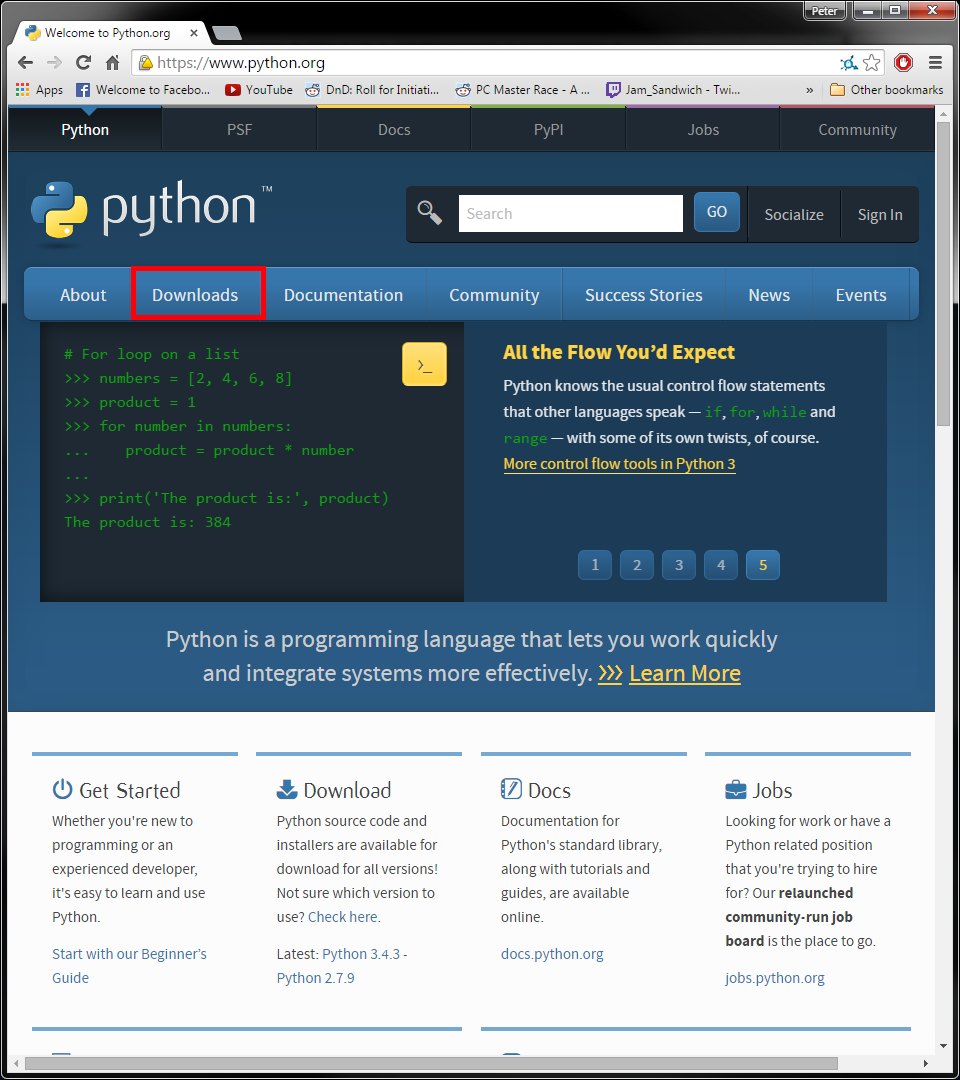
\includegraphics[width=\textwidth]{./Manual/PythonInstall/Part1.png}
\caption{The python home web page} \label{fig:PyISP1}
\end{figure}
\item Under "Download the latest version for windows" click on the Download Python 3.x.x button
\begin{figure}[H]
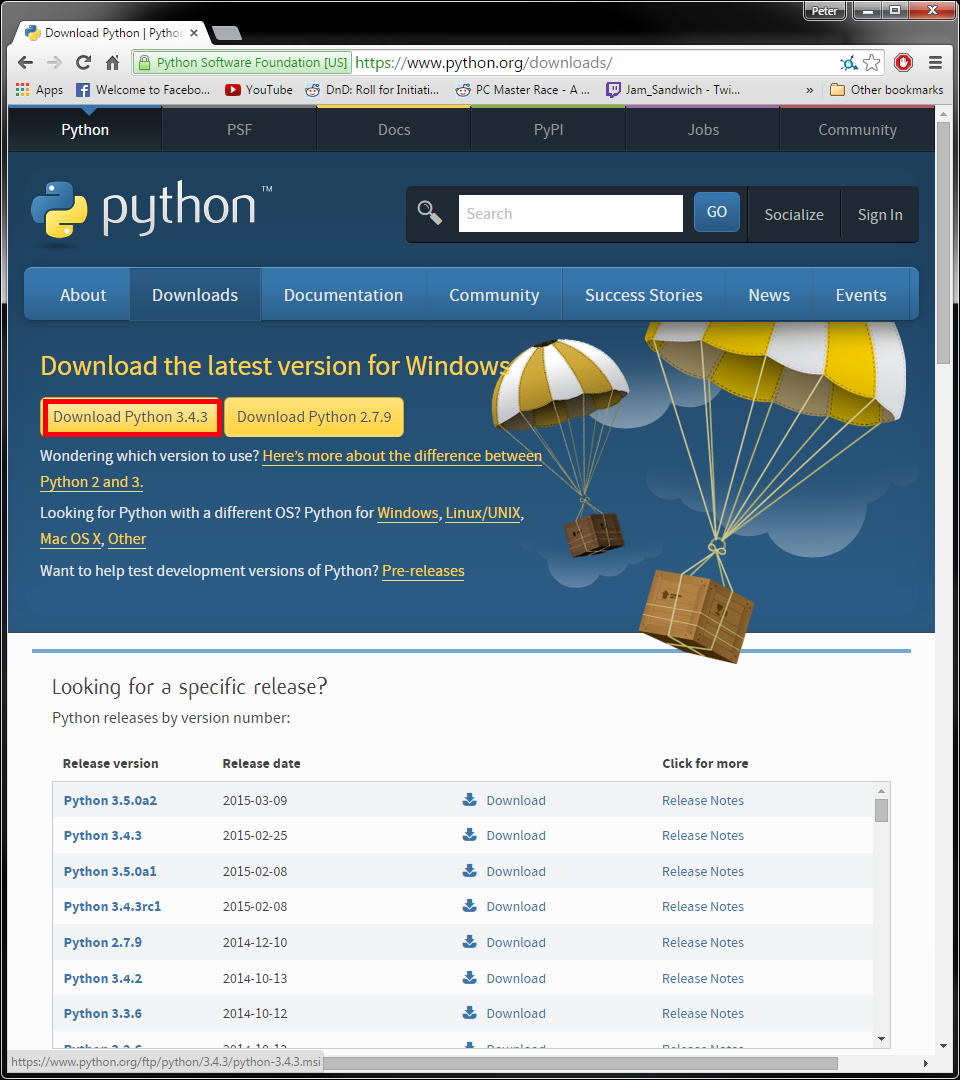
\includegraphics[width=\textwidth]{./Manual/PythonInstall/Part2.png}
\caption{The python downloads page} \label{fig:PyISP2}
\end{figure}
\item Run the .msi file that you have just downloaded
\item you may need to allow windows to run the file as showen
\begin{figure}[H]
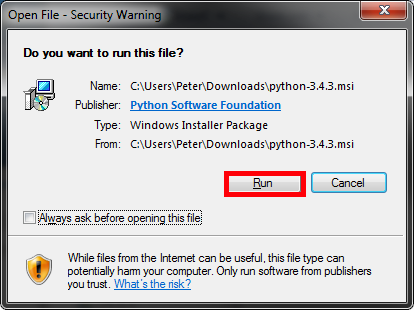
\includegraphics[width=\textwidth]{./Manual/PythonInstall/Part3.png}
\caption{Windows Security Waring} \label{fig:PyISP3}
\end{figure}
\item Select the install for all users option, then press next
\begin{figure}[H]
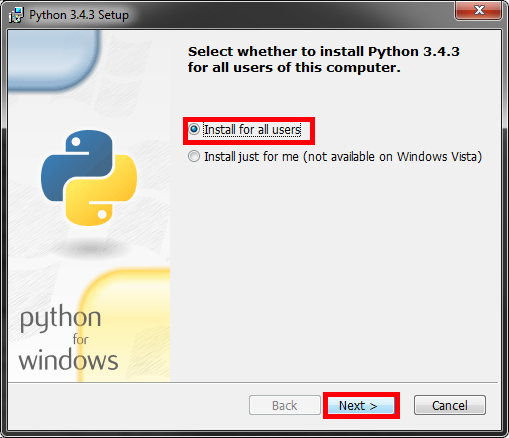
\includegraphics[width=\textwidth]{./Manual/PythonInstall/Part4.png}
\caption{The Python installer} \label{fig:PyISP4}
\end{figure}
\item select a directory for Python to intall in, make a note of this as you will need this when installing PyQt, press nest to continue with the  installation prosses
\begin{figure}[H]
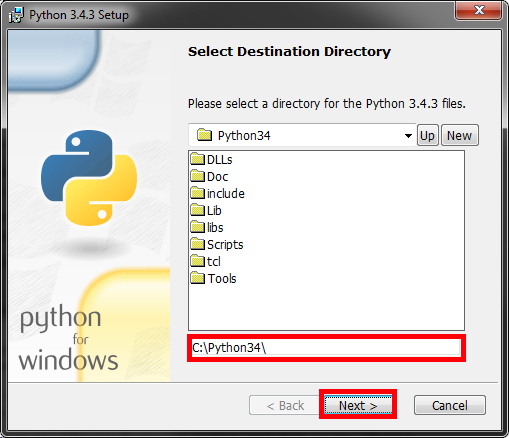
\includegraphics[width=\textwidth]{./Manual/PythonInstall/Part5.png}
\caption{The Python installer} \label{fig:PyISP5}
\end{figure}
\item Make sure that you use the defult installation and press next button
\begin{figure}[H]
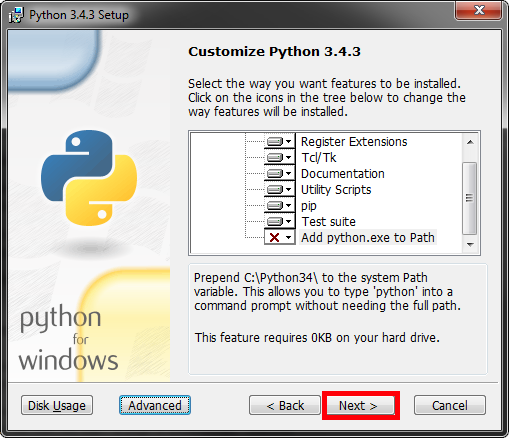
\includegraphics[width=\textwidth]{./Manual/PythonInstall/Part6.png}
\caption{The Python installer} \label{fig:PyISP6}
\end{figure}
\item Allow the installer a few moments to install
\item Python is now installed, just press finish to close the installer
\begin{figure}[H]
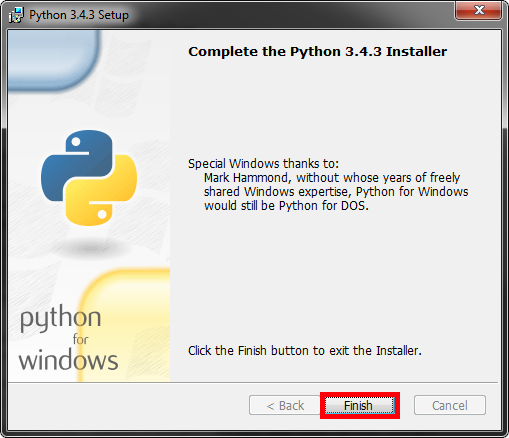
\includegraphics[width=\textwidth]{./Manual/PythonInstall/Part7.png}
\caption{The Python installer} \label{fig:PyISP6}
\end{figure}
\end{enumerate}

\subsubsection{Installing PyQt}
\begin{enumerate}
\item In an internet browser go to the river bank computing web site found at http://www.riverbankcomputing.com/software/pyqt/download
\item Scroll down to the "Binary Packages" section and click on one of the higlited linked depending on for operating system(OS), if you are unsure of you OS then chouse the 32 bit installer
\begin{figure}[H]
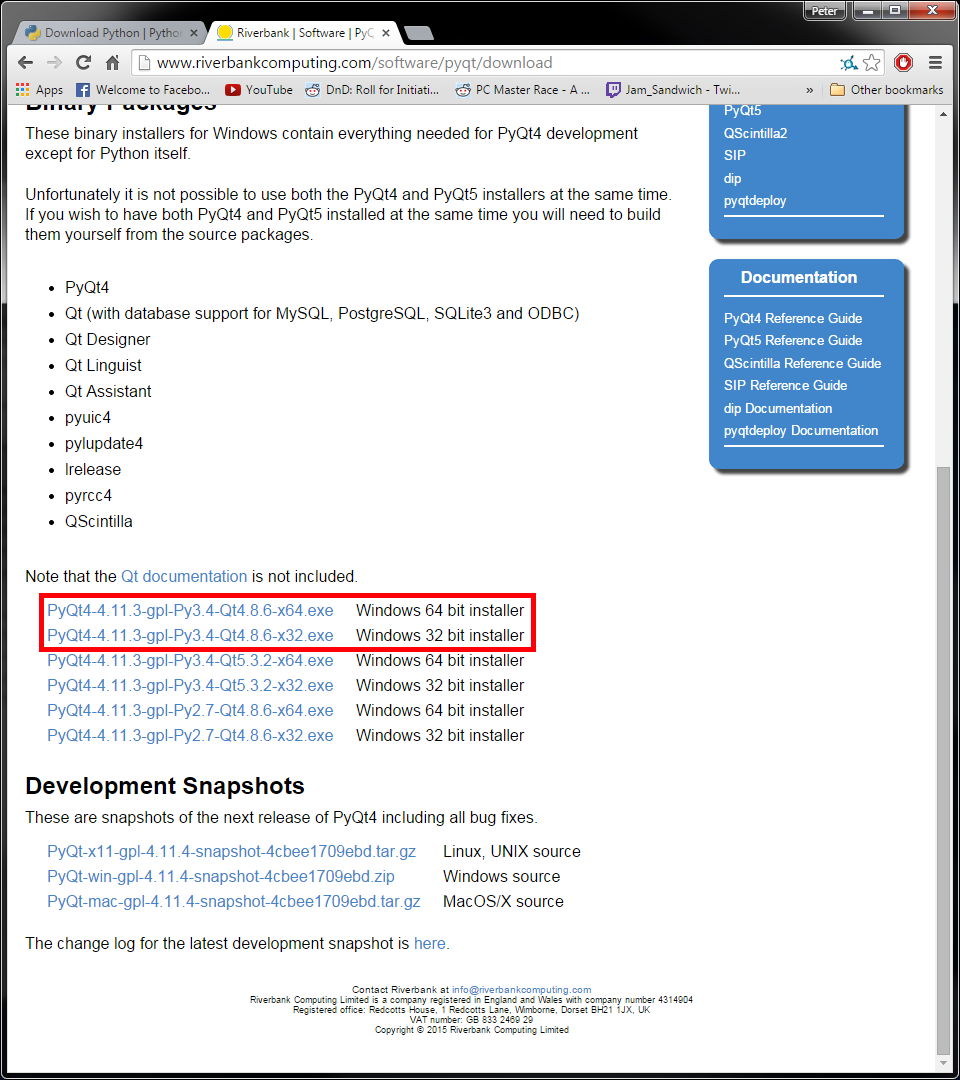
\includegraphics[width=\textwidth]{./Manual/PyQtInstall/Part1.png}
\caption{The River Bank Computing webpage} \label{fig:PyQtISP1}
\end{figure}
\item Run the .exe file that just downloaded and follow the on screen instructions
\item you may need to allow windows to run the file as showen
\begin{figure}[H]
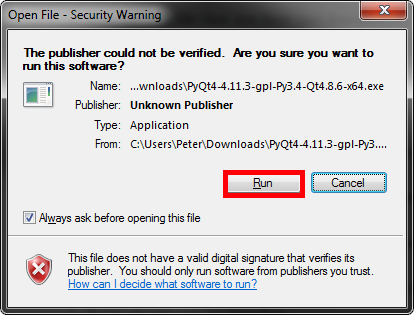
\includegraphics[width=\textwidth]{./Manual/PyQtInstall/Part2.png}
\caption{Windows Security Waring} \label{fig:PyQtISP2}
\end{figure}
\item Click next on the setup wizard
\begin{figure}[H]
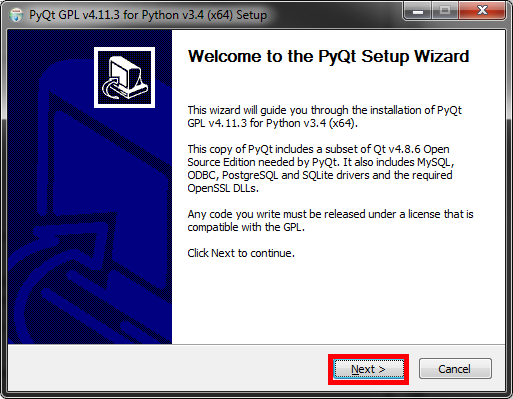
\includegraphics[width=\textwidth]{./Manual/PyQtInstall/Part3.png}
\caption{PyQt setup wizard} \label{fig:PyQtISP3}
\end{figure}
\item read the license agreement and if you agree click the I Agree button, if you chouse not to agree the system will not work
\begin{figure}[H]
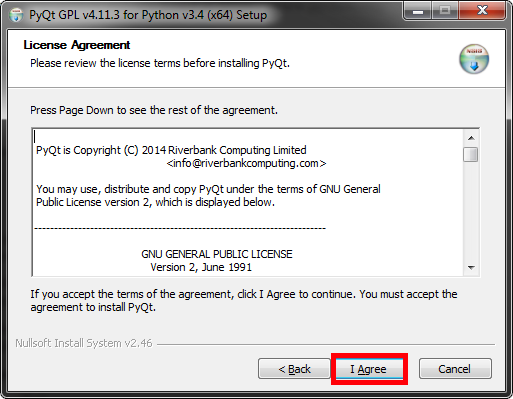
\includegraphics[width=\textwidth]{./Manual/PyQtInstall/Part4.png}
\caption{PyQt setup wizard} \label{fig:PyQtISP4}
\end{figure}
\item Make sure that you install the the full package of PyQt and click the next button
\begin{figure}[H]
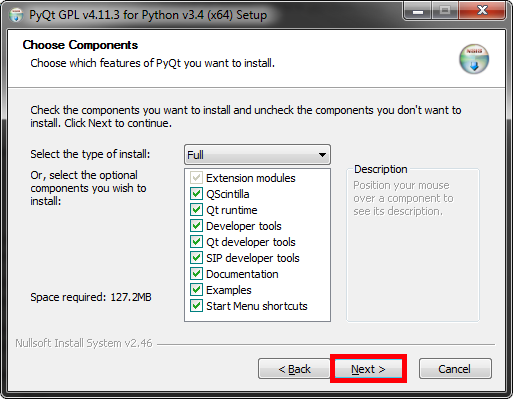
\includegraphics[width=\textwidth]{./Manual/PyQtInstall/Part5.png}
\caption{PyQt setup wizard} \label{fig:PyQtISP5}
\end{figure}
\item Use the directory that have used for the Python install earlyer, then click install
\begin{figure}[H]
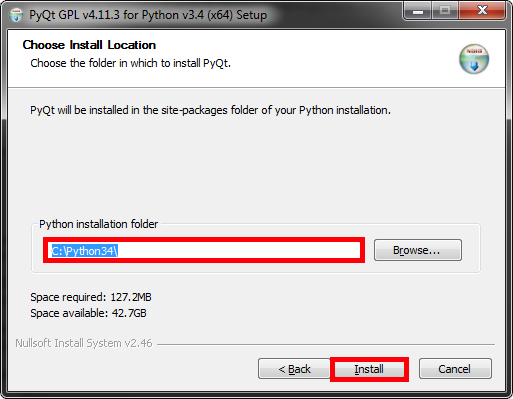
\includegraphics[width=\textwidth]{./Manual/PyQtInstall/Part6.png}
\caption{PyQt setup wizard} \label{fig:PyQtISP6}
\end{figure}
\item Alow PyQt a few moments to install
\item The click the finsish button to close the setup wizard
\begin{figure}[H]
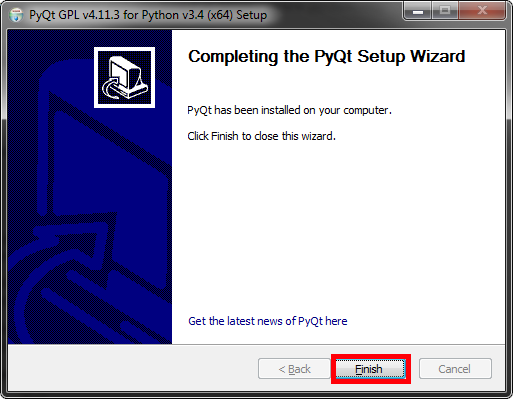
\includegraphics[width=\textwidth]{./Manual/PyQtInstall/Part7.png}
\caption{PyQt setup wizard} \label{fig:PyQtISP7}
\end{figure}
\end{enumerate}

\subsection{System Installation}
\begin{enumerate}
\item In an internet browser go to https://github.com/24697/COMP4Coursework/releases
\item Then click on the TeamCambridgeDatabaseManagerV1.0.zip link
\begin{figure}[H]
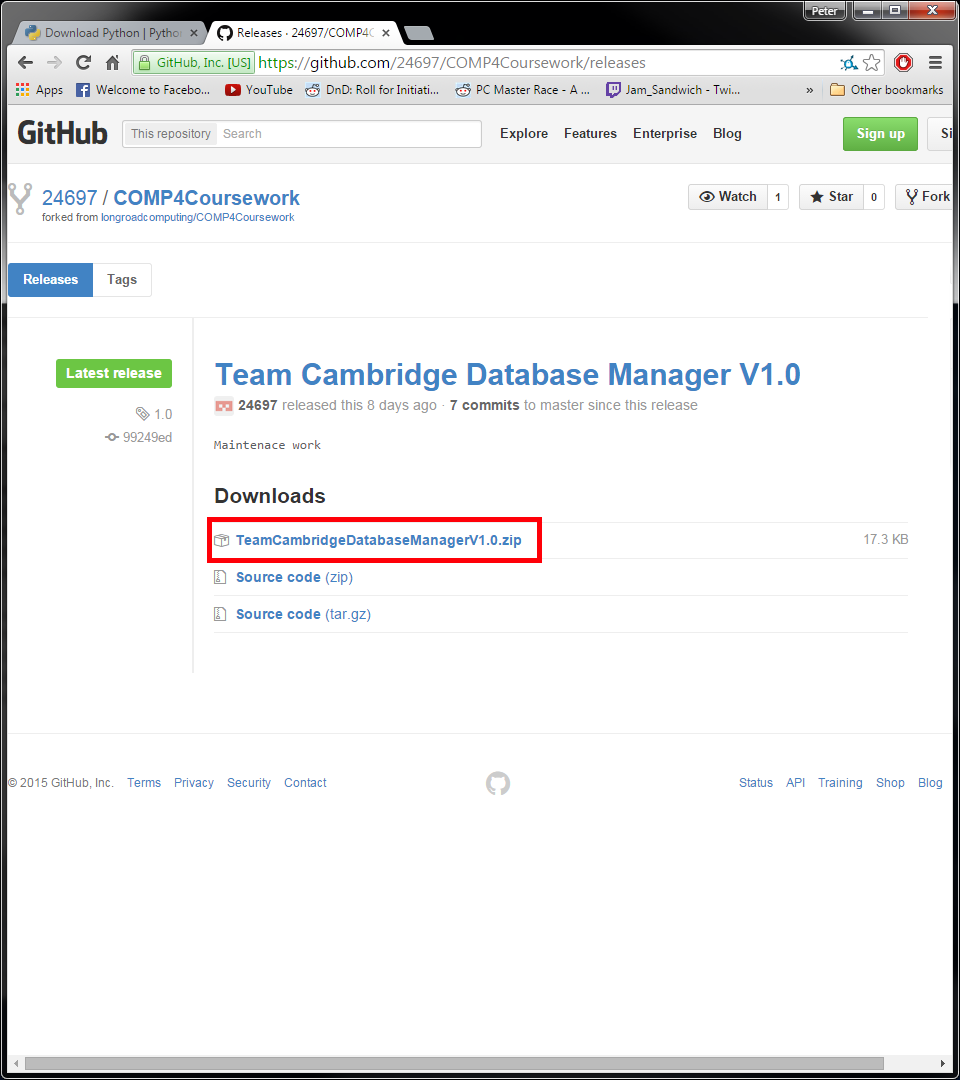
\includegraphics[width=\textwidth]{./Manual/SystemInstall/Part1.png}
\caption{The Github relice page} \label{fig:SyIsP1}
\end{figure}
\item Open the downloaded file in windows explorer
\begin{figure}[H]
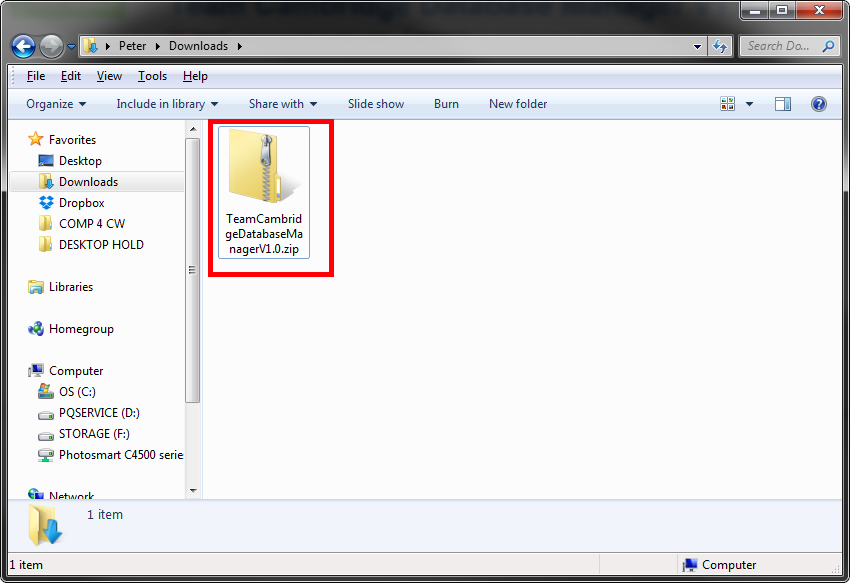
\includegraphics[width=\textwidth]{./Manual/SystemInstall/Part2.png}
\caption{Widows Explorer} \label{fig:SyIsP2}
\end{figure}
\item Then click on the "extract all files" button in the top left hand of the window
\begin{figure}[H]
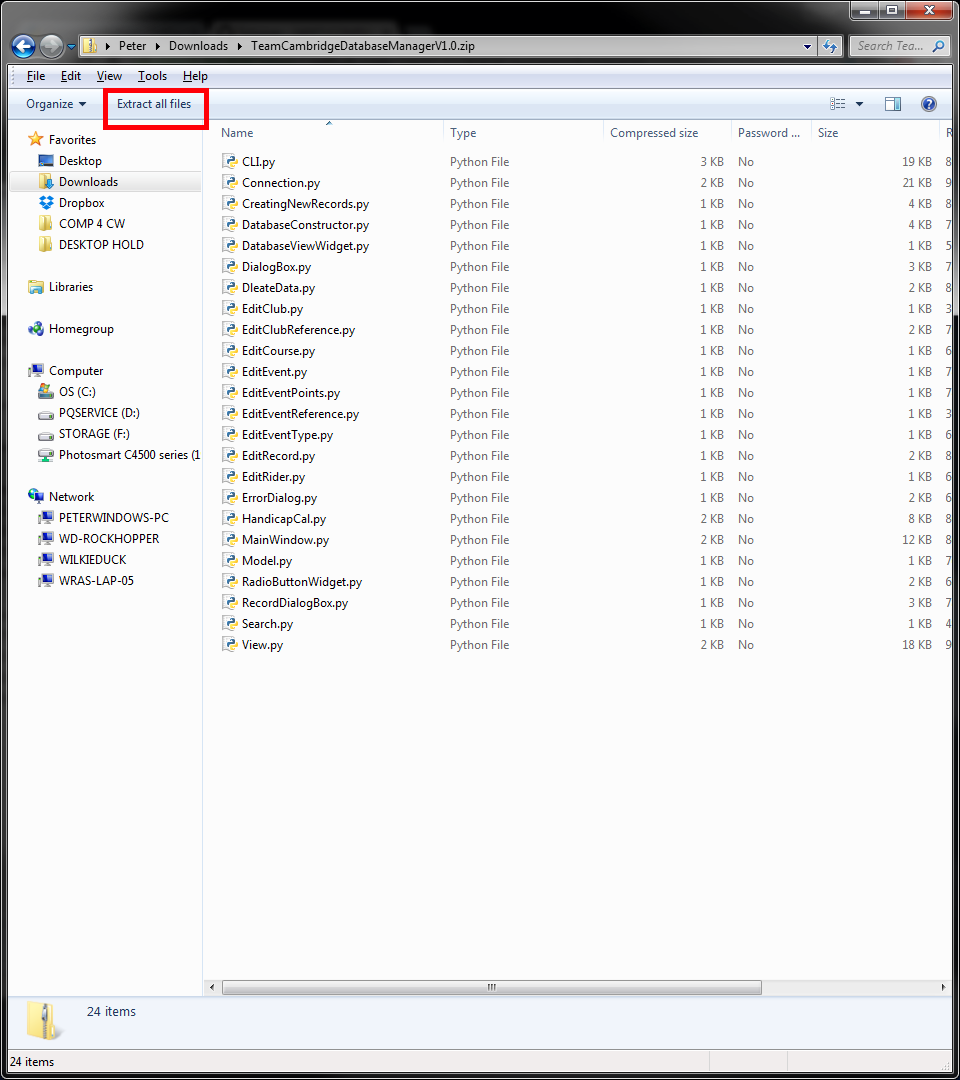
\includegraphics[width=\textwidth]{./Manual/SystemInstall/Part3.png}
\caption{Windows Explorer} \label{fig:SyIsP3}
\end{figure}
\item then select a directory where you wish the application to be installed, then click extract
\begin{figure}[H]
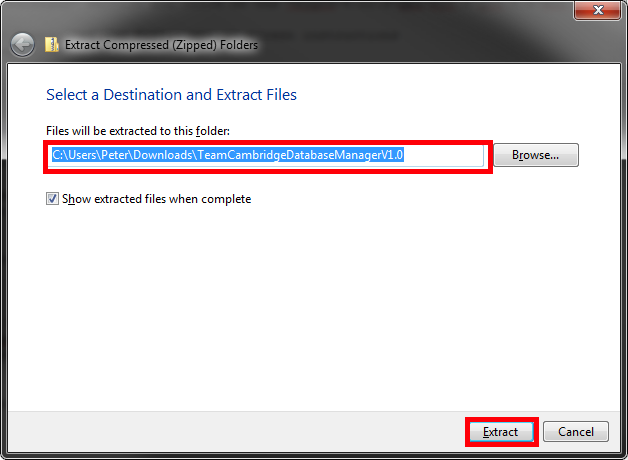
\includegraphics[width=\textwidth]{./Manual/SystemInstall/Part4.png}
\caption{Windows Explorer} \label{fig:SyIsP4}
\end{figure}
\item Browse to the location that you have just chosen, and run the  DatabaseConstructor.py file
\begin{figure}[H]
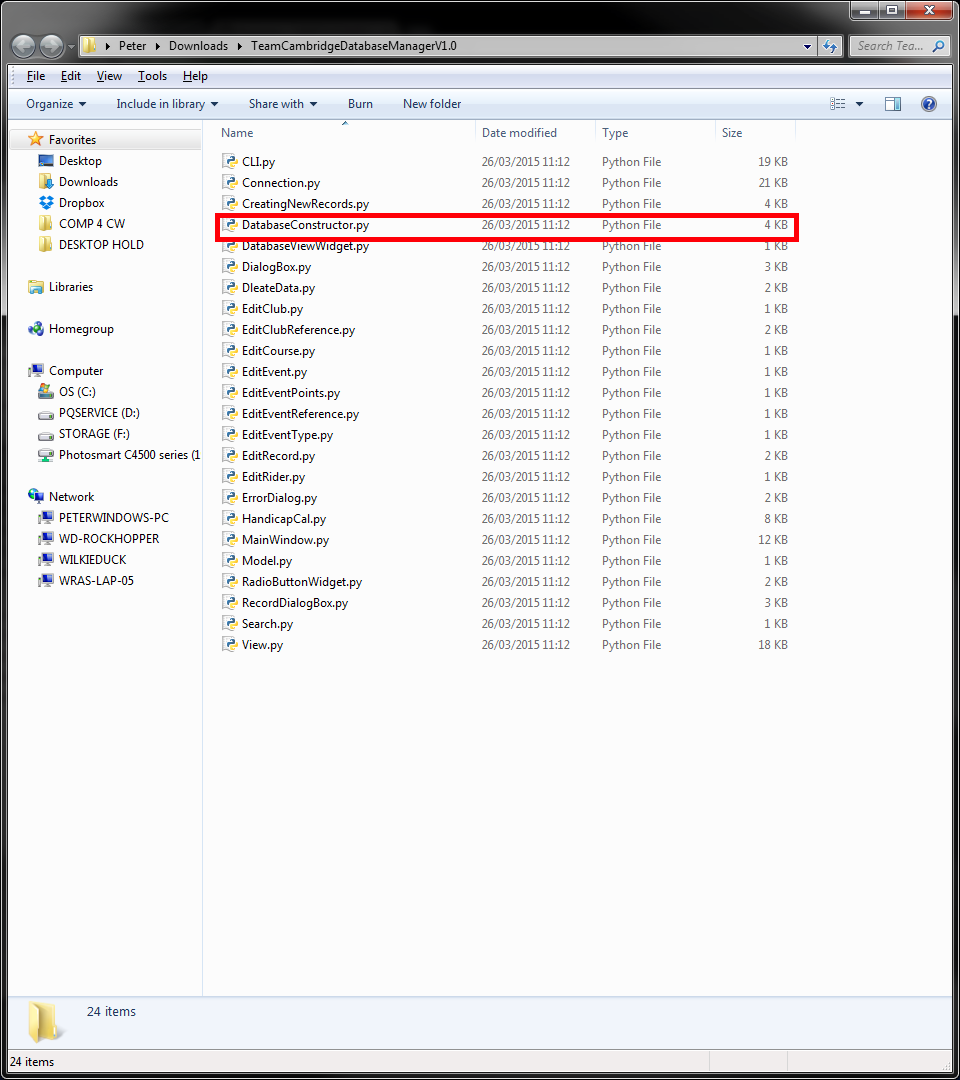
\includegraphics[width=\textwidth]{./Manual/SystemInstall/Part5.png}
\caption{Windows Explorer} \label{fig:SyIsP5}
\end{figure}
\end{enumerate}
\subsection{Running the System}
To run the system you will need to run the MainWindow.py file
\section{Tutorial}

\subsection{Introduction}
This tutorial is structured in a FAQ style so that the user can find how to complease a spesific tast aswell as find the overall squence of how to add an event and then records to the event while being able to look up the spesifics of each section. 

\subsection{Assumptions}
I am assuming that the user has a basic understanding of the time tile system and basic skills with a computer.
\subsection{Tutorial Questions}

\subsubsection{What is the process of loading the database}
When you run the MainWindow.py file a file dialogue window will open, navigate to the file where the TeamCambridge.db file is located and double click on it. the database should now be loaded.

If yo miss-click on another file then you will need to close the application and start again.

\subsubsection{What is the process of adding a rider?}
\begin{enumerate}
\item Navigate to the Rider table by clicking on the "Tables" button on the menu bar, then click the "Rider" button
\item Now click on the "Add Data" button
\item Fill the "Forename" and "Surname" line edits with appropriate data and click the "OK" button
\item The data will be added to the database and the database will be saved automatically.
\end{enumerate}

Note: If one or both of the fields are not filled an error messages will appear when the "OK" button is pressed

\subsubsection{What is the process of adding a club?}
\begin{enumerate}
\item Navigate to the Club table by clicking on the "Tables" button on the menu bar, then click the "Club" button
\item Now click on the "Add Data" button
\item Fill the "Club" line edit with appropriate data and click the "OK" button
\item The data will be added to the database and the database will be saved automatically.
\end{enumerate}

Note: If  the field is not filled an error messages will apper when the "OK" button is pressed

\subsubsection{What is the process of adding a course?}
\begin{enumerate}
\item Navigate to the Course table by clicking on the "Tables" button on the menu bar, then click the "Course" button
\item Now click on the "Add Data" button
\item Fill the "Course Code" and "Course Distance" line edits with appropriate data and click the "OK" button
\item The data will be added to the database and the database will be saved automatically.
\end{enumerate}

Note: If  any of the fields are not filled an error messages will appear when the "OK" button is pressed

\subsubsection{What is the process of connecting a club to a rider?}
\begin{enumerate}
\item Find the RiderID of the rider that you wish to connect a club to
\item Switch to the Club table and find the ClubID of the club that you wish to connect to the rider
\item Switch to the Club Reference table
\item Click on the "Add Data" button on the tool bar
\item Put the RiderID and ClubID in the appropriate line edits and fill the rest of the line edits appropriately
\item Click the "OK" button, the database will be updated wit the new information and saved
\end{enumerate}
\subsubsection{What is the process of adding an event?}
\begin{enumerate}
\item Find the CourseID of the course you wish to use for the event, if you need to add a course not see above to fin how to add a course to the database
\item Switch to the Event table and click on the "Add Data" button on the tool bar
\item Place the CourseID in the "CourseID" line edit and fill the rest of the line edits appropriately
\item Click the "OK" button, the database will be updated wit the new information and saved
\end{enumerate}
\subsubsection{What is the process of adding a record to an event?}
\begin{enumerate}
\item Find the EventID of the Event that you wish to add a Record to
\item Find the RiderID of the Rider that you wish to use in the Record
\item Switch to the Record table and click on the "Add Data" button
\item Put the EventID and RiderID in the matching line edit, and fill the rest of the line edits appropriately
\item Find the RiderID of the rider that you wish to connect a club to
\end{enumerate}
\subsubsection{What is the process of adding an event with records and points from beginning to end?}
\begin{enumerate}
\item First you will need to add a Course(see above for details)(if the course you want to use is already added to the database then skip this instruction)
\item Second you will need to add an Event and link it to the course you have just made(see above for details)
\item Now make sure that you have riders made to add the event(see above for details)
\item Now create a record and link it to the event that you have just made and make a new record to each rider you wish to connect to the  event(see above for details)
\item Finally for each record create a Event Points entry
\end{enumerate}

\subsection{Saving}
The system saves to the TeamCambridge.db file each time data is added or deleted from the database, so you will not need to save the database before closing the application.
\subsection{Limitations}
There are few limitation of the current system, one is that the edit function is not implemented in the main application, this was due to lack of time however the edit function was implemented in the CLI so you can edit data using the CLI.
\section{Error Recovery}
There are some error with the current system 
\subsection{Error 1}

\subsection{Error 2}

\section{System Recovery}

\subsection{Backing-up Data}
To Back up the data you will need to make a copy of the TeamCambridge.db file. I would recommend that several copies of the file are made on separate storage devises. For example if all the copies of the .db file are on one storage device and that device fails then recovering the .db file can be expensive or impossible as if you keep copies on different storage devices then if one device fail then you will have a back up available.

Making regular updates would also be good for data recover, I would recommend making a backup every week and keeping the last 3 weeks of back ups replacing the oldest back up each week. 
\subsection{Restoring Data}
In the unlikely event of data loss or corruption all you will need to do is copy the most recent working copy of the TeamCambidge.db file to the same file as the application and run the application as normal.

\stopcontents[UserManual]
